\chapter{Visualisation implementation of the Improved Kepler Visualisation Tool
(IKVT)}\label{C:sd}
This chapter discusses the implementation of the visulisation using the designs
discussed in the previous chapter to fulfill the requirements for this project.
It details the tools used, the deliverable features
produced, and the problems encountered. 

\section{Tools and artifacts used}
\subsection{Dataset used}
The dataset for this project is a comma separated values file (CSV) that
contains all of the data pertaining to the Exoplanets. At runtime this dataset
is read into the system and an Exoplanet object is created for each element and
contains all of the information from the dataset record.

%possibly discuss how a real database could be used instead
\subsection{Integrated Development Environment (IDE)}
The IDE used for this project is one that is provided with Processing. This IDE
provided all of the tools and functionality that were required to effectively
implement the solution for this project. Another option that could have been
taken was to use Eclipse with the processing package and external libraries
imported. However I found that the processing IDE was entirely suitable for the
majority of my needs creating the visualisation. The key things that I did not
have access to with this choice was the Eclipse Debugger and JUnit tests. ~   
\subsection{Keyboard and Mouse System}
In addition to Processing in the main system there was an additional opensource
library required for effective user interface components, this library was
called ControlP5 \cite{controlp5}. This library is a customisable and intuitive interactive
user interface. It allows for easy creation of visually appealing and precisely
layed out interactive GUI components.

\subsection{Microsoft Kinect sensor system}
For the version of the IKVT system that uses the Kinect sensor for user
interaction two additional libraries were required to integrate the hardware
with Processing, these were:
\begin{enumerate}
 \item NITE \cite{nite}
 \item SimpleOpenNi \cite{simpleopenni}
\end{enumerate}
These libraries provided drivers to run the Kinect sensor in Processing as well
as basic gesture recognition and body tracking. However as the libraries were
opensource due to the official Microsoft Kinect SDK not being compatible with
Processing, the gesture recognition was not as user friendly or effective as the
official libraries. The effect of this was that the gesture tracking used in the
system had to be created sup-optimally from the opensource libraries. 

\section{Implementation of IKVT}

IKVT displays all 2234 exoplanets
in the Kepler exoplanets dataset \cite{dataset}. Each of these exoplanets are
represented as coloured
ellipses, of which the colour and size are representative of the exoplanets
temperature and size respectively. IKVT displays all of these exoplanets as if
they are orbiting a single star which in reality would result in planetary
collisions but in the visualisation provides users with a way to effectively
make observations and comparisons about each of the exoplanets in a single
view. 

There are two panels that make up the visualisation, the visualisation panel,
and the control panel. The visualisation panel is where all of the exoplanets
are displayed as well as text boxes describing the state of the visualisation to
keep the user informed. The control panel contains all of the interactive
components that the user can use to change the state of the visualisation. The
components it contains are; two text areas that cane be used interchangeably to
display information about selected planets, four range sliders (Figure: \ref{fig:sliders}) that are used to
filter the exoplanets as discussed previously, and eight buttons to toggle the
state of the visualisations. These buttons are "Sort by KOI", "Sort by Temp",
"Sort by Size", "Sort by ESI", "Change View", "Suns Habitable Zone", "Pause",
and "Unsort" as shown in Figure: \ref{fig:buttons}. 

\begin{figure}[H]
  \centering
      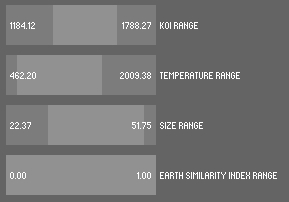
\includegraphics[width=0.6\textwidth]{images/sliders.jpg}
  \caption{Panel of interactive range sliders}
  \label{fig:sliders}
\end{figure}

\begin{figure}[H]
  \centering
      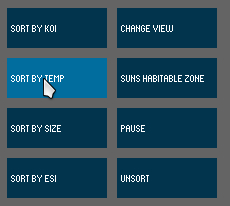
\includegraphics[width=0.6\textwidth]{images/buttons.jpg}
  \caption{Panel of interactive buttons}
  \label{fig:buttons}
\end{figure}

Detailed information can be accessed about each exoplanet by clicking on them in the main visualisation window to
make a selection. To do this a user can click on any of the orbiting exoplanets.
The effect of this selection is that a text box will have further textual
information about the selected exoplanet appended to it to provide the user with
more detailed information \ref{fig:textBoxes}. When a user is unable to accurately select an
exoplanet due to clustering or
overlapping of exoplanets they can move the camera around in space to gain a
better viewing position with which to make their selection. If this is not
enough, the user can use a set of range filters to filter the exoplanets
displayed as in Figure: \ref{fig:zoomFilter}. The attributes that can be filtered by are are Kepler Object of Interest number (KOI),
temperature, size, and Earth Similarity Index (ESI). These filters allow for
users to fine tune the exoplanets they wish, thus allowing them to work
with small multiples rather than the entire dataset. A further effect of using these filters is that a zooming effect occurs as less exoplanets are displayed. This zooming occurs each time the filters are changed as the exoplanets spread out vertically so that it allows more space between them to make selections.

\begin{figure}[H]
  \centering
      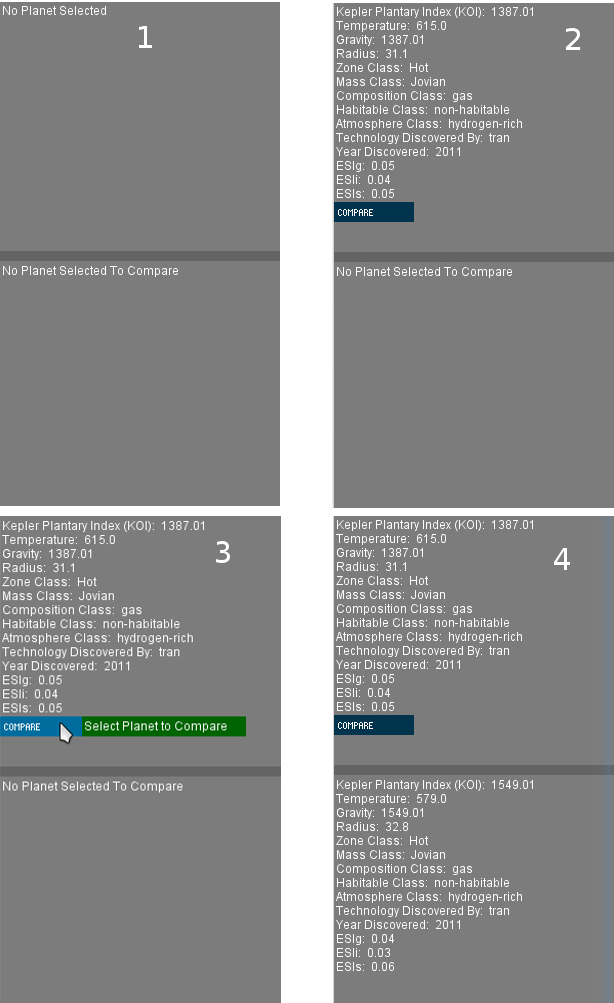
\includegraphics[width=0.9\textwidth]{images/textBoxes.jpg}
  \caption{Text boxes in each possible state}
  \label{fig:textBoxes}
\end{figure}

\begin{figure}[H]
  \centering
      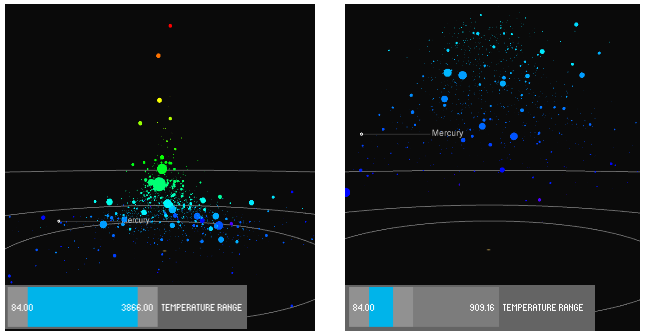
\includegraphics[width=0.8\textwidth]{images/zoomFilter.png}
  \caption{TODO~}  
    \label{fig:zoomFilter}
\end{figure}

\begin{figure}[H]
  \centering
      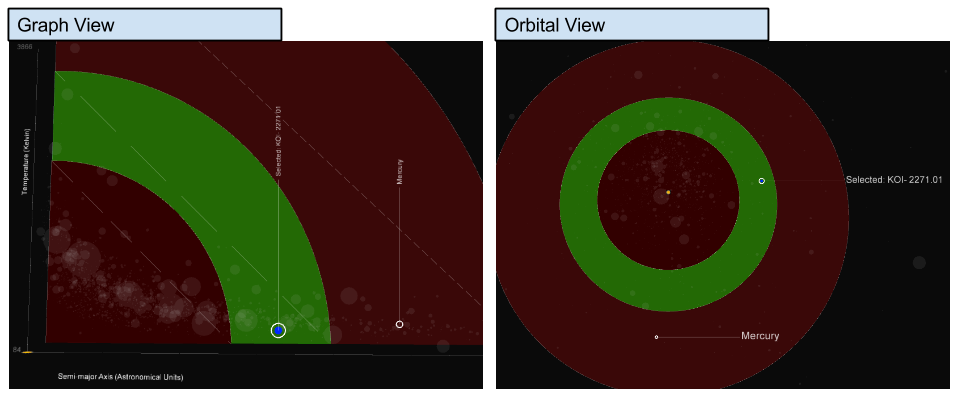
\includegraphics[width=1\textwidth]{images/habitable.png}
  \caption{TODO~}  
    \label{fig:habitable}
\end{figure}

\subsubsection{Interaction Panel}
Description of navigation window
\begin{figure}[H]
  \centering
      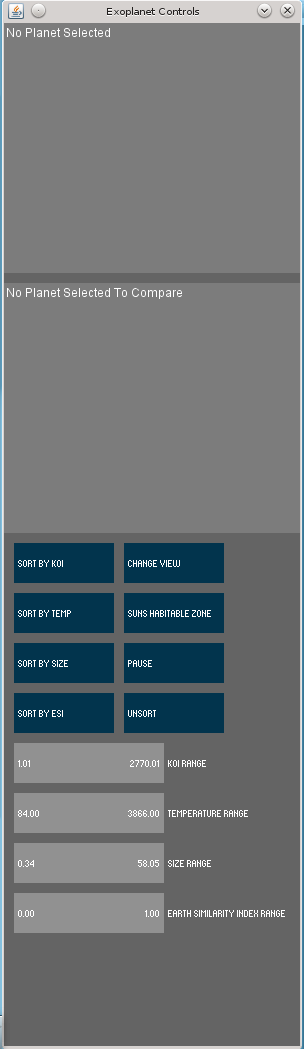
\includegraphics[width=0.3\textwidth]{images/nav.png}
  \caption{Navigation Panel Overview}
  \label{fig:nav}
\end{figure}

Due to the need for increased user interaction with the visualisation a window
is required to house the buttons, range selectors, and text areas. These
elements are needed as the different methods that users can use to interact with
the visualisation need to be visually apparent to ensure that the system can be
easily used without prior experience. A way to do this is to provide clearly
labeled interactive elements and tooltips explaining what they
do. These tooltips are widely used as a method of informing a
user about the purpose of an item by hovering over it. This removes the need to
click on a button to discover its effect.


In addition to this, the screen needs to display the user in relation to the
screen, an effective way to do this is to display a washed out representation of
themselves in the background of the visualisation.


\subsubsection{Spacial arrangement of components}
As the majority of the interaction and movement of visualisation elements occurs
in the center of the window it caused a aspect ratio that was not suitable . It
was BETTER~ to use 2 vertical columns to view and control the visualisation as
it had a higher aspect ratio which allowed more of the content to be seen on the
screen at once thanks to the fact that the majority of computer screens have a
wide ratio.

\begin{figure}[H]
  \centering
      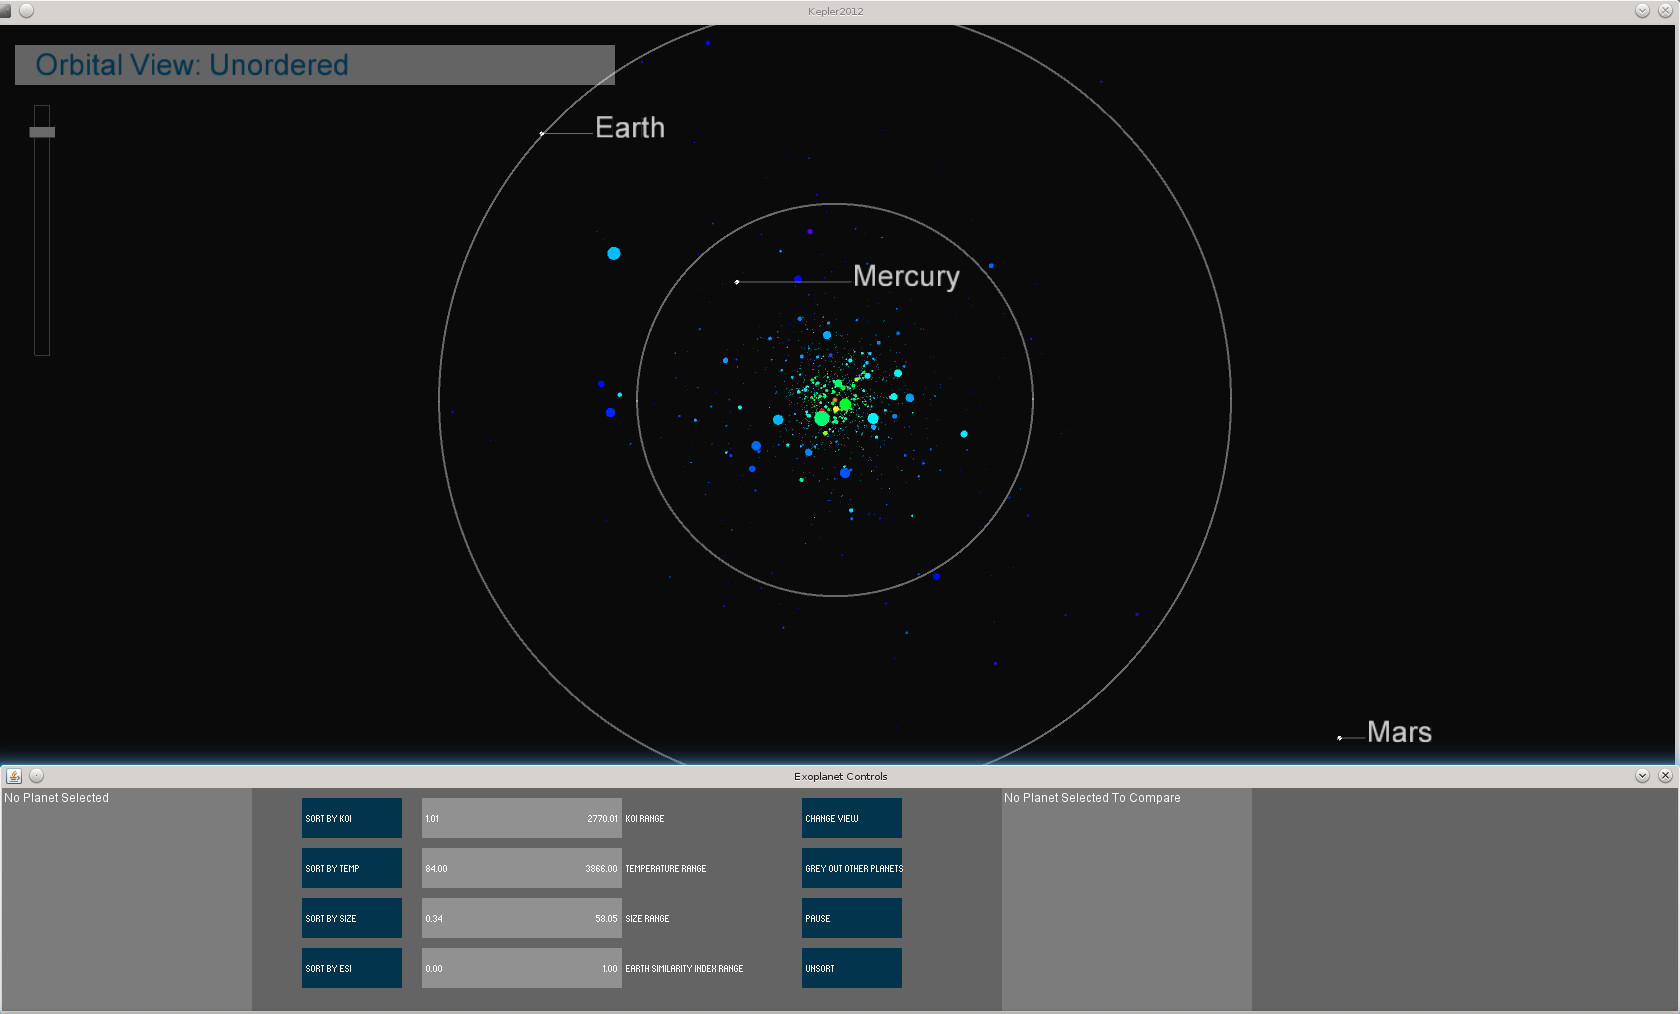
\includegraphics[width=0.8\textwidth]{images/layout_horizontal.jpg}
  \caption{Original Horizontal Layout}  
        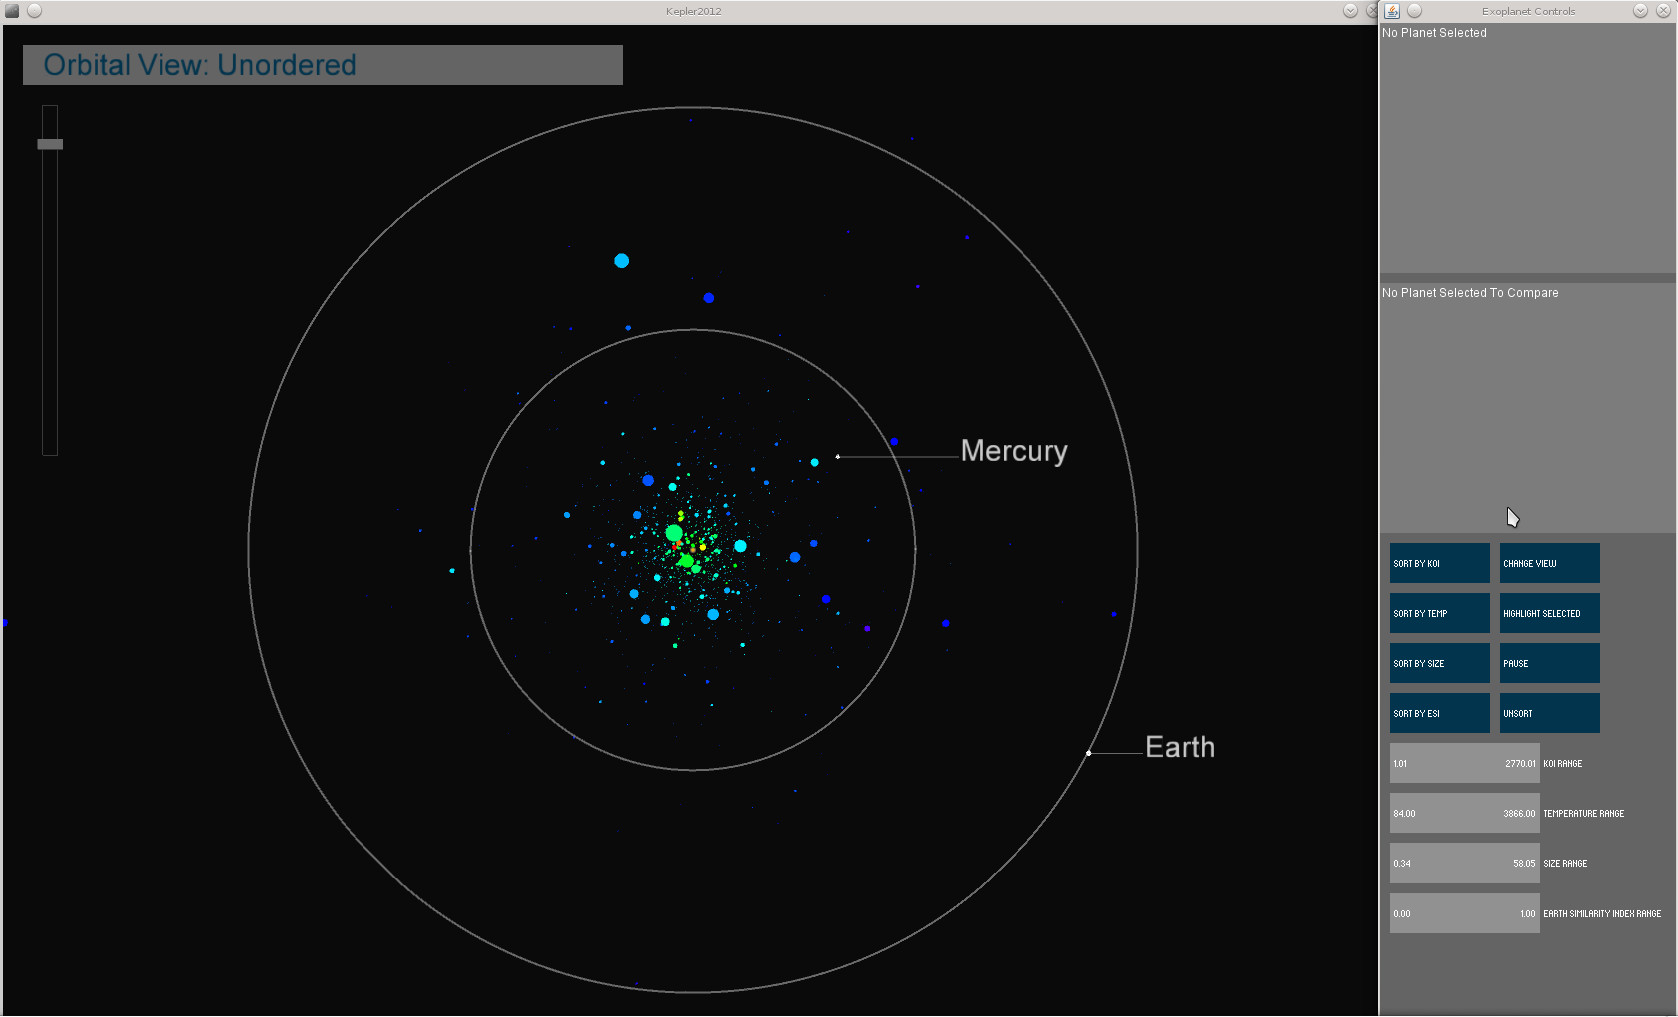
\includegraphics[width=0.8\textwidth]{images/layout_vertical.jpg}
  \caption{Improved Vertical Layout}
\end{figure}


\section{Problems encountered}
Due to the number of elements that needed to be displayed on screen at any one
time (ie 2234 exoplanets), the load placed on a system is very high due to the
need to render 2234 eclipses to represent the planets. This uncovered a bug in
the processing library in which the memory use of the visualisation would
periodically increase until it crashed due to an out of memory exception. After
much experimentation of how to overcome this issue, I discovered that rather
than trying to render a native ellipse shape in processing, if I instead
rendered
a Scalable Vector Graphic this bug would not manifest. 
\\\\
Libraries used for gesture detection in kinect are opensource in order to work
with processing did not have decent detection
\\\\
Using the Processing framework meant using a non industrial???~ IDE that had
many bugs, for example when undoing multiple times in a row the file being
modified would periodically become corrupted by lines of code being taken away
or inserted into the wrong locations. The solution to this issue was to ensure
that I regularly committed any changes to my version controlled system on Github
\cite{github}. Doing this meant that if at any time a file became corrupted I
could easily see the changes in the file when compared against the precious
commit and manually fix the file. 
\\\\
As this project builds upon a previous system much of the existing code and
execution flow needs to be modified. This requires understanding of how the
system was originally built and designed. Because this system does not have any
unit or integration tests, going ahead without a comprehensive knowledge of the
core functionality would be have led to ineffective planning and errors being
introduced into the system.
%Making use of tall of the data
